\documentclass[11pt,a4paper,sans]{moderncv}        % possible options include font size ('10pt', '11pt' and '12pt'), paper size ('a4paper', 'letterpaper', 'a5paper', 'legalpaper', 'executivepaper' and 'landscape') and font family ('sans' and 'roman')

%\usepackage{tikz,mwe}
\usepackage{tikz}
\newcommand{\tikzcircle}[2][, fill={rgb:black,2;white,2}]{\tikz[baseline=-0.7ex]\draw[#1,radius=#2] (2,0) circle ;}%
\usepackage{footmisc}


\newcommand*{\xingsocialsymbol}    {{\small\faXing}~} 
\newcommand*{\gitlabsocialsymbol}  {{\small\faGitlab}~} 
\newcommand*{\skypesocialsymbol}   {{\small\faSkype}~} 
\newcommand*{\stackoverflowsocialsymbol} {{\small\faStackOverflow}~}
\newcommand*{\bitbucketsocialsymbol} {{\small\faBitbucket}~}
\newcommand*{\orcidsocialsymbol} {{\small\faOrcid}~}
\newcommand*{\researchgatesocialsymbol}  {{\small\faResearchgate}~}
\newcommand*{\googlescholarsocialsymbol}  {{\small\faGoogleScholar}~}
\newcommand*{\telegramsocialsymbol}  {{\small\faTelegram}~}
\newcommand*{\whatsappsocialsymbol} {{\small\faWhatsapp}~}
\newcommand*{\bornsymbol} {{\small\faAsterisk}~}  

% moderncv themes
\moderncvstyle{classic
}          % style options are 'casual' (default), 'classic', 'oldstyle' and 'banking'
\moderncvcolor{blue}                                % color options 'blue' (default), 'orange', 'green', 'red', 'purple', 'grey' and 'black'
%\renewcommand{\familydefault}{\sfdefault}         % to set the default font; use '\sfdefault' for the default sans serif font, '\rmdefault' for the default roman one, or any tex font name
%\nopagenumbers{}                                  % uncomment to suppress automatic page numbering for CVs longer than one page

% character encoding
\usepackage[utf8]{inputenc}                       % if you are not using xelatex ou lualatex, replace by the encoding you are using
%\usepackage{CJKutf8}                              % if you need to use CJK to typeset your resume in Chinese, Japanese or Korean

% adjust the page margins
\usepackage[scale=0.75]{geometry}
%\setlength{\hintscolumnwidth}{3cm}                % if you want to change the width of the column with the dates
%\setlength{\makecvtitlenamewidth}{10cm}           % for the 'classic' style, if you want to force
%the width allocated to your name and avoid line breaks. be careful though, the length is normally
%calculated to avoid any overlap with your personal info; use this at your own typographical
%risks...

%Show labels in the bibliography
\makeatletter
\renewcommand*\bibliographyitemlabel{\@biblabel{\arabic{enumiv}}}
\makeatother
\renewcommand{\refname}{Last update: \today \vspace{2mm}}

\makeatletter
% commands from moderncvstylebanking.sty to have the title
% from that style
\newcommand*{\maketitlesymbol}{%
    {~~~{\rmfamily\textbullet}~~~}}% the \rmfamily is required to force Latin Modern fonts when using sans serif, as OMS/lmss/m/n is not defined and gets substituted by OMS/cmsy/m/n
%   internal command to add an element to the footer
%   it collects the elements in a temporary box, and checks when to flush the box
\newsavebox{\maketitlebox}%
\newsavebox{\maketitletempbox}%
\newlength{\maketitlewidth}%
\newlength{\maketitleboxwidth}%
\newif\if@firstmaketitleelement\@firstmaketitleelementtrue%
%   adds an element to the maketitle, separated by maketitlesymbol
%   usage: \addtomaketitle[maketitlesymbol]{element}
\newcommand*{\addtomaketitle}[2][\maketitlesymbol]{%
  \if@firstmaketitleelement%
    \savebox{\maketitletempbox}{\usebox{\maketitlebox}#2}%
  \else%
    \savebox{\maketitletempbox}{\usebox{\maketitlebox}#1#2}\fi%
  \settowidth{\maketitleboxwidth}{\usebox{\maketitletempbox}}%
  \ifnum\maketitleboxwidth<\maketitlewidth%
    \savebox{\maketitlebox}{\usebox{\maketitletempbox}}%
    \@firstmaketitleelementfalse%
  \else%
    \flushmaketitle{}\\%
    \savebox{\maketitlebox}{#2}%
    \savebox{\maketitletempbox}{#2}%
    \settowidth{\maketitleboxwidth}{\usebox{\maketitlebox}}%
    \@firstmaketitleelementfalse\fi}
%   internal command to flush the maketitle
\newcommand*{\flushmaketitle}{%
  \strut\usebox{\maketitlebox}%
  \savebox{\maketitlebox}{}%
  \savebox{\maketitletempbox}{}%
  \setlength{\maketitleboxwidth}{0pt}}
\renewcommand*{\maketitle}{%
  \setlength{\maketitlewidth}{0.8\textwidth}%
  \hfil%
  \parbox{\maketitlewidth}{%
    \centering%
    % name and title
    \namestyle{\@firstname~\@lastname}%
    \ifthenelse{\equal{\@title}{}}{}{\titlestyle{~|~\@title}}\\% \isundefined doesn't work on \@title, as LaTeX itself defines \@title (before it possibly gets redefined by \title) 
    % detailed information
    \addressfont\color{color2}%
    \ifthenelse{\isundefined{\@addressstreet}}{}{\addtomaketitle{\addresssymbol\@addressstreet}%
      \ifthenelse{\equal{\@addresscity}{}}{}{\addtomaketitle[~--~]{\@addresscity}}% if \addresstreet is defined, \addresscity and \addresscountry will always be defined but could be empty
      \ifthenelse{\equal{\@addresscountry}{}}{}{\addtomaketitle[~--~]{\@addresscountry}}%
      \flushmaketitle\@firstmaketitleelementtrue\\}%
    \collectionloop{phones}{% the key holds the phone type (=symbol command prefix), the item holds the number
      \addtomaketitle{\csname\collectionloopkey phonesymbol\endcsname\collectionloopitem}}%
    \ifthenelse{\isundefined{\@email}}{}{\addtomaketitle{\emailsymbol\emaillink{\@email}}}%
    \ifthenelse{\isundefined{\@homepage}}{}{\addtomaketitle{\homepagesymbol\httplink{\@homepage}}}%
    \collectionloop{socials}{% the key holds the social type (=symbol command prefix), the item holds the link
      \addtomaketitle{\csname\collectionloopkey socialsymbol\endcsname\collectionloopitem}}%
    \ifthenelse{\isundefined{\@extrainfo}}{}{\addtomaketitle{\@extrainfo}}%
    \flushmaketitle}\\[2.5em]}% need to force a \par after this to avoid weird spacing bug at the first section if no blank line is left after \maketitle

\renewcommand*{\namefont}{\Huge\bfseries\upshape}
\renewcommand*{\titlefont}{\Huge\mdseries\upshape}
\renewcommand*{\addressfont}{\normalsize\mdseries\upshape}
\renewcommand*{\quotefont}{\large\slshape}

% styles
\renewcommand*{\namestyle}[1]{{\namefont\textcolor{color1}{#1}}}
\renewcommand*{\titlestyle}[1]{{\titlefont\textcolor{color2!85}{#1}}}
\renewcommand*{\addressstyle}[1]{{\addressfont\textcolor{color1}{#1}}}
\renewcommand*{\quotestyle}[1]{{\quotefont\textcolor{color1}{#1}}}

\renewcommand*{\makecvtitle}{%
  % recompute lengths (in case we are switching from letter to resume, or vice versa)
  \recomputecvlengths%
  \maketitle%
  % optional quote
  \ifthenelse{\isundefined{\@quote}}%
    {}%
    {{\centering\begin{minipage}{\quotewidth}\centering\quotestyle{\@quote}\end{minipage}\\[2.5em]}}%
  \par}% to avoid weird spacing bug at the first section if no blank line is left after \maketitle}

\makeatother

% personal data
\name{Robert}{Krug}
\title{Curriculum Vitae}     
\extrainfo{Citizenship: Austrian \hspace{1mm} \tikzcircle{2pt} \hspace{1mm} Date of birth: $12/07/1981$}                 % optional, remove / comment the line if not wanted                          % optional, remove / comment the line if not wanted
\address{Faberstr. 8c}{81373 Munich}{Germany}% optional, remove / comment the line if not wanted; the "postcode city" and and "country" arguments can be omitted or provided empty
\phone[mobile]{+49 152 02407853}                   % optional, remove / comment the line if not wanted
\phone[fixed]{+49 711 811-92523}                    % optional, remove / comment the line if not wanted
\email{krug.r1@gmail.com}                               % optional, remove / comment the line if not wanted
\social[linkedin][linkedin.com/in/robert-krug-74ab62164]{robert-krug}

%\homepage{www.kth.se/profile/rkrug?l=en}                         % optional, remove / comment the line if not wanted
\photo[64pt][0.4pt]{photo}                       % optional, remove / comment the line if not wanted; '64pt' is the height the picture must be resized to, 0.4pt is the thickness of the frame around it (put it to 0pt for no frame) and 'picture' is the name of the picture file
%\quote{Some quote}                                 % optional, remove / comment the line if not wanted

% to show numerical labels in the bibliography (default is to show no labels); only useful if you make citations in your resume
%\makeatletter
%\renewcommand*{\bibliographyitemlabel}{\@biblabel{\arabic{enumiv}}}
%\makeatother
%\renewcommand*{\bibliographyitemlabel}{[\arabic{enumiv}]}% CONSIDER REPLACING THE ABOVE BY THIS

% bibliography with mutiple entries
\usepackage{multibib}
\usepackage{enumitem}
\newcommand{\MYhref}[3][blue]{\href{#2}{\color{#1}{#3}}}%

\newcites{book,misc}{{Books},{Others}}
%----------------------------------------------------------------------------------
%            content
%----------------------------------------------------------------------------------
\begin{document}
%\begin{CJK*}{UTF8}{gbsn}                          % to typeset your resume in Chinese using CJK
%-----       resume       ---------------------------------------------------------
\makecvtitle

\newcommand\logocity[3][]{
  \tikz[baseline=(n.center)]
  \node(n)[align=center,inner sep=0,outer sep=0]{\includegraphics[#1]{#2}\\[1ex]#3};
}
\begin{picture}(0,0)
  \put(0,44){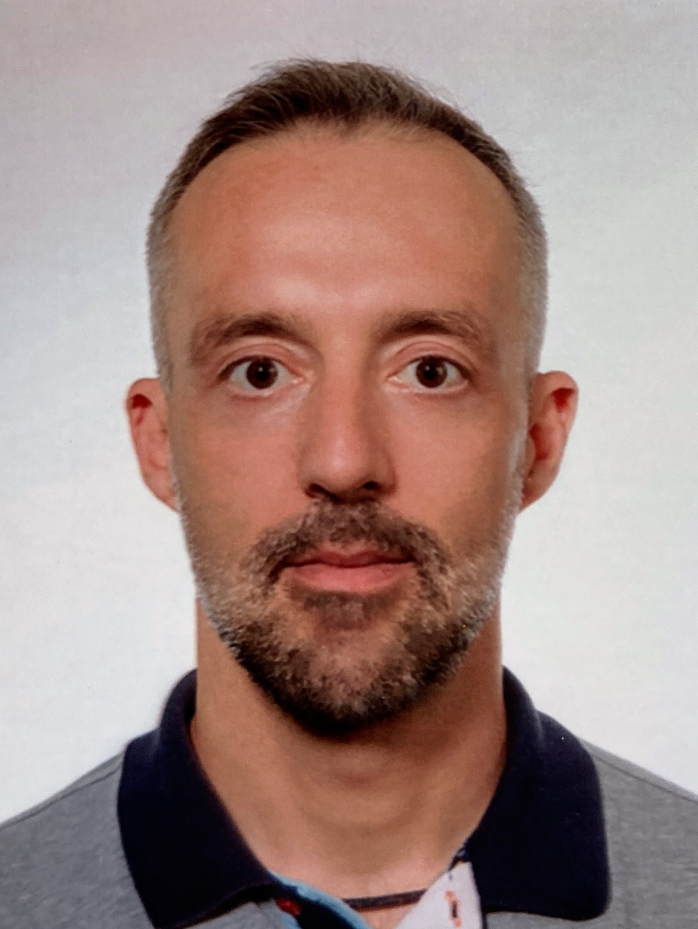
\includegraphics[scale=0.03]{photo.png}}
\end{picture}

\vspace{-5mm}
\section{Current Position}

\cventry{$2018$--present}{Research engineer}{}{}{R\&D Robotics, Bosch Corporate Research, Stuttgart Area, Germany}{}
\begin{itemize}[leftmargin=1cm, itemsep=-2pt]
  \item Closed-loop multi-modal policy learning for industrial robot manipulation 
  \item Reinforcement learning for robot manipulation tasks~\MYhref{https://argmin.lis.tu-berlin.de/papers/20-hoppe-IROS.pdf}{\underline{(paper)}}
  \item Model-based manipulator control with learned residuals~\MYhref{https://www.roboticsproceedings.org/rss18/p066.pdf}{\underline{(paper)}}
  \item Impedance-controlled insertion primitives for industrial assembly~\MYhref{https://www.sciencedirect.com/science/article/abs/pii/S0736584523001126}{\underline{(paper)}}

\end{itemize}

\section{Previous Positions}

\cventry{$2017$--$2018$}{Post-doctoral researcher}{}{}{Robotics, Perception and Learning lab,
  KTH Royal Institute of Technology, Stockholm, Sweden}{}
\begin{itemize}[leftmargin=1cm, itemsep=-2pt]
    \item Scientific coordinator of project FACT (Factories of the Future)
    \item Assisted telemanipulation~\MYhref{https://ieeexplore.ieee.org/document/8594457}{\underline{(paper)}}~\MYhref{https://www.youtube.com/watch?v=B3ybwrGH-e4}{\underline{(video)}}
    \item Skill-based robotic manipulation~\MYhref{https://www.ijcai.org/proceedings/2018/0003.pdf}{\underline{(paper)}}
  \end{itemize}

\cventry{$2014$--$2017$}{Post-doctoral researcher}{}{}{AASS Research Center,
  {\"O}rebro University, {\"O}rebro, Sweden}{}
  \begin{itemize}[leftmargin=1cm, itemsep=-2pt]
    \item Trajectory optimization for robot fleet navigation~\MYhref{https://ieeexplore.ieee.org/document/8594118}{\underline{(paper)}}
    \item Hierarchical control for robot manipulation~\MYhref{https://www.diva-portal.org/smash/get/diva2:1044259/FULLTEXT01.pdf}{\underline{(paper)}}~\MYhref{https://www.youtube.com/watch?v=_xM9RQAbxEY}{\underline{(video)}} 
    \item Robot grasping with tactile feedback~\MYhref{https://ieeexplore.ieee.org/abstract/document/7487130}{\underline{(paper)}}
    \item Analytical grasp analysis~\MYhref{https://www.diva-portal.org/smash/get/diva2:1163511/FULLTEXT01.pdf}{\underline{(paper)}}
  \end{itemize}
\section{Education}
\cventry{$2009$--$2014$}{PhD in Control Theory}{}{}{AASS
  Research Center, {\"O}rebro University}{\textit{Thesis topic:} ``Optimization-based Robot Grasp
  Synthesis and Motion Control''.\\ \textit{Supervisors:} Prof. Achim J. Lilienthal and Dr. Dimitar
  N. Dimitrov.}

\cventry{$2001$--$2009$}{MSc in Mechatronics in Mechanical
  Engineering}{}{}{Graz University of Technology}{\textit{Thesis topic:} ``Dev. of a Flexible Handling- and Assemblysystem for Short Cycle
  Times''.\\ \textit{Supervisor:} Prof. Michael Hofbaur.}

\newpage

\section{Skills}

\cventry{}{Python \& Pytorch}{}{\textit{Experience:} ML application development for 5+ years}{}{}
\cventry{}{C++}{}{\textit{Experience}: Real-time robot control framework development for 5+ years}{}{}
\cventry{}{MATLAB}{}{\textit{Experience}: Algorithm development for 5+ years}{}{}
\cventry{}{ROS}{}{\textit{Experience}: Application development on various platforms for 10+ years}{}{}
\cventry{}{DevOps}{}{\textit{Experience}: Using standard tools (Git, Docker, Jenkins, ...) for 10+ years}{}{}

\section{Teaching}

\cventry{$2018$}{Advanced Individual Course in Computer Science}{}{Masters level course}{KTH Stockholm}{Instructor}

\cventry{$2016$}{Robot Control}{}{Masters level course}{{\"O}rebro University}{Instructor}
%\footnotetext{Lecture notes available at:
%  \url{http://www.aass.oru.se/Research/Learning/rkg_dir/course_rc_2016.html}}

\cventry{$2011$}{Sensors and Sensing}{}{Masters level course}{{\"O}rebro University}{TA for Dr. Boyko Iliev}

\cventry{$2010$--$2011$}{Artificial Intelligence in Mobile Robots}{}{Masters level
  course}{{\"O}rebro University}{TA for Prof. Alessandro Saffiotti}

\cventry{$2005$--$2007$}{Principles of Dynamics}{}{Undergraduate course}{Graz University of
Technology}{TA for Prof. Andr\'{e}s Kecskem\'{e}thy \& Prof. Walter Sextro}

\cventry{$2005$--$2007$}{Principles of Statics}{}{Undergraduate course}{Graz University of
Technology}{TA for Prof. Andr\'{e}s Kecskem\'{e}thy \& Prof. Walter Sextro}

\section{Mentoring}

\cventry{}{Moritz Schneider}{}{Phd Co-Advisor}{R\&D Robotics, Bosch Corporate Research}{}

\cventry{}{Sathiya Ramesh, Moritz Reuss, Sanjeev Kumar}{}{Masters Advisor}{R\&D Robotics, Bosch Corporate Research}{}

\cventry{}{Shahbaz Kader, Michael Welle, Ioanna Mitsioni}{}{PhD Co-Advisor}{KTH Stockholm}{}

\cventry{}{Jens Lundell,  Jo\~ao Salvado}{}{PhD Co-Advisor}{{\"O}rebro University}{}

\cventry{}{Bowen Kuang, Dennis Malmgren, Alvin Sing Teck Lee}{}{Masters Advisor}{KTH Stockholm}{}

\cventry{}{Marcus A. Johansson, Chittaranjan Swaminathan}{}{Masters Advisor}{{\"O}rebro University}{}

\section{Publications}

An up-to-date publication list of peer-reviewed conference and journal papers, as well as patents is available on Google Scholar\footnotemark.
\footnotetext{\url{https://scholar.google.se/citations?user=OZNzz9gAAAAJ\&hl=en}}
\vspace{4mm}
\newpage
\nocite{*}
\bibliographystyle{IEEEtran}%plain,unsrt,alpha,abbrv,acm,apalike
\bibliography{Publications}



% \section{Languages}
% \cvitemwithcomment{German}{Native speaker}{}
% \cvitemwithcomment{English}{Proficient}{}
% \cvitemwithcomment{Swedish}{Basic}{}


% % Publications from a BibTeX file using the multibib package
% \section{Publications}
% \nocitebook{book1,book2}
% \bibliographystylebook{plain}
% \bibliographybook{publications}                   % 'publications' is the name of a BibTeX file
% \nocitemisc{misc1,misc2,misc3}
% \bibliographystylemisc{plain}
% \bibliographymisc{publications} 



\end{document}
